\documentclass{article}

% Encodings, page setup, paragraph formatting, font
\usepackage[top=0.9in, bottom=1in, left=1.5in, right=1.5in]{geometry}
\usepackage[icelandic]{babel}
\usepackage[T1]{fontenc}
\usepackage[sc]{mathpazo}
\usepackage[parfill]{parskip}
\usepackage{cancel}
\usepackage{comment}
% Tables and lists
\usepackage{booktabs,tabularx}
\usepackage{multirow}
\usepackage{enumerate}
\usepackage{adjustbox}
\usepackage{multicol}
\usepackage{enumitem}
\usepackage{xcolor}
% Math
\usepackage{amsmath, amsfonts, amssymb, amsthm}
\usepackage{gensymb}
% Graphics
\usepackage{graphicx}
\usepackage{forest}
\usepackage{tikz}
\usetikzlibrary{positioning, shapes, arrows.meta}
% Code environment
\usepackage{listingsutf8}
\definecolor{commentcolor}{RGB}{0, 128, 0} % Grænn
\definecolor{keywordcolor}{RGB}{0, 0, 255}   % Blár
\definecolor{stringcolor}{RGB}{163, 21, 21}      % Dökkrauður
\definecolor{numbercolor}{RGB}{128, 0, 128}      % Fjólublár
\definecolor{identifiercolor}{RGB}{0, 0, 0}      % Svartur

\lstset{
    language=Java,
    basicstyle=\ttfamily,
    keywordstyle=\color{keywordcolor}\bfseries,
    commentstyle=\color{commentcolor},
    identifierstyle=\color{identifiercolor},
    stringstyle=\color{stringcolor},   
    showstringspaces=false,
    numbers=left,
    numberstyle=\tiny\color{gray},
    tabsize=2,
    breaklines=true,
    columns=fullflexible,
    keepspaces=true,
    inputencoding=utf8, 
    extendedchars=true,  
    literate=
        {á}{{\'a}}1
        {ð}{{\dh}}1
        {é}{{\'e}}1
        {í}{{\'i}}1
        {ó}{{\'o}}1
        {ú}{{\'u}}1
        {ý}{{\'y}}1
        {þ}{{\th}}1
        {æ}{{\ae}}1
        {ö}{{\"o}}1
        {Á}{{\'A}}1
        {Ð}{{\DH}}1
        {É}{{\'E}}1
        {Í}{{\'I}}1
        {Ó}{{\'O}}1
        {Ú}{{\'U}}1
        {Ý}{{\'Y}}1
        {Þ}{{\TH}}1
        {Æ}{{\AE}}1
        {Ö}{{\"O}}1,
}

% Restin af forskriftinni
\usepackage[pdftex,bookmarks=true,colorlinks=true,pdfauthor={Hafsteinn Einarsson},linkcolor=blue,urlcolor=blue]{hyperref}

% Hyphenation
\hyphenpenalty=5000
% Page and section numbering
\setcounter{secnumdepth}{-1} 
\pagenumbering{gobble}

\title{Tölvutækni og forritun Lokapróf}
\author{brj46 }
\date{Nóvember 2024}

\begin{document}

\maketitle

\vspace {7em}
\begin{center}

\includegraphics[width=0.7\textwidth]{3d.jpg}
\end{center}

\newpage
\section*{Hvað Þarf Ég Að Kunna?}

\begin{itemize}
    \item[$\square$] Varpanir (tvívíðar og þrívíðar) (töluleg rök)
    \item[$\square$] Hreyfanleg líkön (WebGl) (Render-Föll)
    \item[$\square$] Endurskinslíkön (Phong lýsingarlíkanið) (útreikningar með dofnun)
    \item[$\square$] Mynsturvörpun (Texture mapping t.d. repeat og \text{CLAMP\_TO\_EDGE}) Ójafnhliða síun
    \item[$\square$] GLSL og litaraforritun (Hnúta- og bútalitarar) (Hreyfing og litabreytingar)
    \item[$\square$] Ýmis atriði í tölvugrafík (Homogeneous hnit) (þríhyrnaröðun)(Skuggakort)
    \item[$\square$] Aukaverkefni (Geislasmölun vs Phong) (Dofnun og birtustýring)
\end{itemize}

\newpage

\section{Mín lausn við prófinu 2023}

\subsection{Varpanir}
\subsubsection{a.} Á myndinni er gefin upphafsstaða á húsi í tvívídd. Neðra vinstra horn þess er i (1, 2).

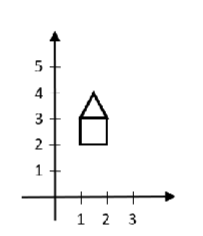
\includegraphics[scale = 0.9]{mynd2023a.png}

Teiknið mynd af stöðu hússins eftir þessar samsettu varpanir (hvor liður sjálfstæður). Rökstyðjið í nokkrum orðum hver útkoman er.

\begin{itemize}
    \item[i.] $T(1, 2)*S(1, 2)*T(2,-1)*R(90\degree)$
    \item[ii.] $T(1, 2)*R(90\degree)*S(1,2)*T(-1,-2)$
\end{itemize}

\subsubsection{b.} Sýnið samsetta tvívíða vörpun sem breytir ferningnum í fyrri myndinni yfir í
ferhyrninginn í seinni myndinni. Seinni ferhyrningurinn er með miðpunkt (2,
2), hliðarlengdir 1 og 2, og halli hans er $45\degree$. Rökstyðjið einstakar
grunnvarpanir í samsettu vörpuninni.

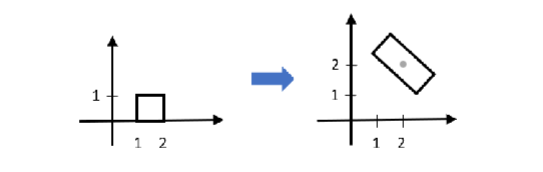
\includegraphics[scale = 0.9]{mynd2023b.png}

\newpage

\subsection{2} WebGl Útfærsla á líkani

Það er til útgáfa af klukku (Continue Time, hönnuður Sander Mulder) sem hefur
þrjá arma eins og venjuleg klukka, en í stað þess að armarnir
snúist allir um sama punkt (þ.e. miðpunkt skífu), þá eru þeir
festir á endann á öðrum armi. Klukkustundararmurinn er
reyndar festur á miðpunkt skífu og snýst um hann eins og á
venjulegri klukku, en mínútuarmurinn er festur á endann á
klukkustundararminum og snýst um þann punkt. Sömuleiðis
er sekúntuarmurinn festur á endann á mínútuarminum og
snýst um hann. Á myndinni hér til hliðar er
klukkustundararmurinn á milli 4 og 5, mínútuarmurinn sýnir
30 og sekúntuarmurinn vísar á 45. Klukkan hér er því
4:30:45.

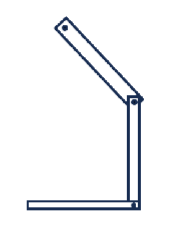
\includegraphics[scale = 0.9]{klukka.png}

Sýnið uppkast að render-falli sem teiknar þessa klukku. Hver armur á að vera
teningur og þið getið gert ráð fyrir að sé búið að hlaða hnúta hans inn í
grafíkminni. Vísarnir eiga að liggja í xy-sléttunni og þeir eiga að snúast rétt,
þannig að fyrir hvern heilan hring sekúntuarmsins snýst mínútuarmurinn sem
svarar einni mínútu (þ.e. 1/60 af heilum hring). Samsvarandi gildir með
klukkustundararminn. Þið eigið bara að uppfæra sekúntuarminn um eina sekúntu í
hverri ítrun render-fallsins (og hina armana samsvarandi). Þetta gefur auðvitað
ekki réttan tíma, en sýnir hreyfingu klukkunnar.
Einbeitið ykkur að því að sýna varpanirnar og teikniföllin í render-fallinu. Þetta
þarf ekki að vera alveg keyranlegur kóði, heldur skiptir meira máli að þið séuð að
hugsa varpanirnar rétt. Útskýrið þess vegna vel einstakar skipanir.

\newpage

\section{3.} Endurskinslíkön

Hér fyrir neðan er líkan með áhorfanda, ljósgjafa og glansandi yfirborði.
Áhorfandinn og ljósgjafinn eru í sömu hæð og beint fyrir ofan sitthvort brotið í
yfirborðinu. Gerið ráð fyrir að notað sé endurskinslíkan Phong án dofnunar til að
búa til lit á yfirborðið.

\begin{center}
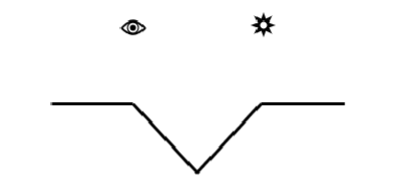
\includegraphics[scale = 0.9]{Endurskin.png}
\end{center}


\subsubsection{a.}Hvar á yfirborðinu er bjartasta \underline{dreif}endurskin (diffuse reflection)? Ef fleiri en
einn staður eru jafnbjartir tilgreinið þá alla björtustu staðina. Rökstyðjið
svarið í nokkrum orðum.

\subsubsection{b.}Hvar á yfirborðinu er bjartasta \underline{depil}endurskin (specular reflection)? Ef fleiri
en einn staður eru jafnbjartir tilgreinið þá alla björtustu staðina. Rökstyðjið
svarið í nokkrum orðum.

\subsubsection{c.}Ef hægt væri að færa ljósið til hliðar (í sömu hæð), eru staðsetningar á ljósinu
sem gefa ekkert depilendurskin á þessu yfirborði? Gerið ráð fyrir að
glansstuðull yfirborðsins sér hár og depillinn sé því lítill. Rökstyðjið svarið.

\subsubsection{d.}Ef ekkert \underline{umhverfis}endurskin (ambient reflection) væri í líkaninu, væri þá
einhver hluti yfirborðsins alveg svartur? Rökstyðjið.


\end{document}